% fig03_pipeline.tex — the closed-form verification pipeline shared by all three
% substrates. Standalone; `make figures` -> figures/fig03_pipeline.pdf.
\documentclass[tikz,border=4pt]{standalone}
\usetikzlibrary{positioning,arrows.meta,shapes.geometric}
\begin{document}
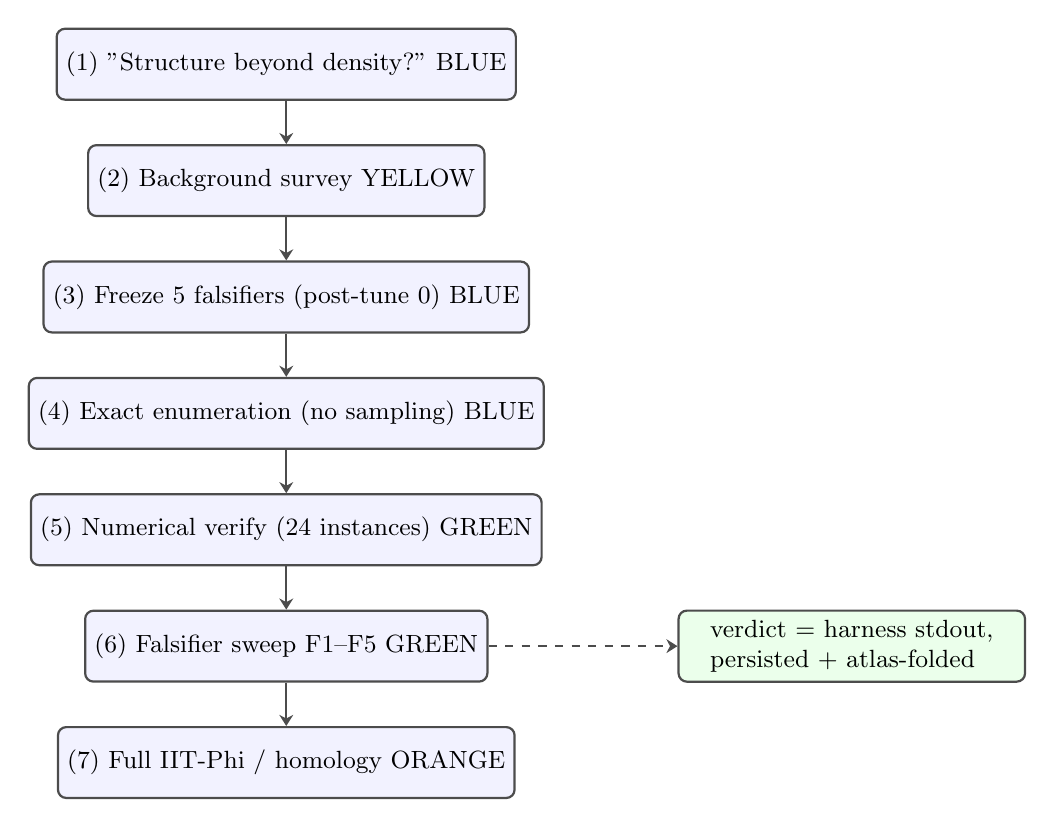
\begin{tikzpicture}[
  font=\small,
  stage/.style = {
    rectangle, rounded corners=3pt, draw=black!70, thick,
    minimum width=4.4cm, minimum height=0.9cm, align=left,
    fill=blue!5,
  },
  arrow/.style = {-{Stealth[length=4pt,width=5pt]}, thick, draw=black!70},
  node distance=0.55cm and 0.9cm,
]
  \node[stage] (s1) {(1) "Structure beyond density?" \hfill BLUE};
  \node[stage, below=of s1] (s2) {(2) Background survey \hfill YELLOW};
  \node[stage, below=of s2] (s3) {(3) Freeze 5 falsifiers (post-tune 0) \hfill BLUE};
  \node[stage, below=of s3] (s4) {(4) Exact enumeration (no sampling) \hfill BLUE};
  \node[stage, below=of s4] (s5) {(5) Numerical verify (24 instances) \hfill GREEN};
  \node[stage, below=of s5] (s6) {(6) Falsifier sweep F1--F5 \hfill GREEN};
  \node[stage, below=of s6] (s7) {(7) Full IIT-Phi / homology \hfill ORANGE};

  \draw[arrow] (s1) -- (s2);
  \draw[arrow] (s2) -- (s3);
  \draw[arrow] (s3) -- (s4);
  \draw[arrow] (s4) -- (s5);
  \draw[arrow] (s5) -- (s6);
  \draw[arrow] (s6) -- (s7);

  % verdict side-note off stage 6
  \node[stage, right=2.4cm of s6, fill=green!8, minimum width=4.4cm] (v)
    {verdict = harness stdout,\\ persisted + atlas-folded};
  \draw[arrow, dashed] (s6.east) -- (v.west);
\end{tikzpicture}
\end{document}
